% Options for packages loaded elsewhere
\PassOptionsToPackage{unicode}{hyperref}
\PassOptionsToPackage{hyphens}{url}
%
\documentclass[
  ignorenonframetext,
  aspectratio=169,
]{beamer}
\usepackage{pgfpages}
\setbeamertemplate{caption}[numbered]
\setbeamertemplate{caption label separator}{: }
\setbeamercolor{caption name}{fg=normal text.fg}
\beamertemplatenavigationsymbolsempty
% Prevent slide breaks in the middle of a paragraph
\widowpenalties 1 10000
\raggedbottom
\setbeamertemplate{part page}{
  \centering
  \begin{beamercolorbox}[sep=16pt,center]{part title}
    \usebeamerfont{part title}\insertpart\par
  \end{beamercolorbox}
}
\setbeamertemplate{section page}{
  \centering
  \begin{beamercolorbox}[sep=12pt,center]{part title}
    \usebeamerfont{section title}\insertsection\par
  \end{beamercolorbox}
}
\setbeamertemplate{subsection page}{
  \centering
  \begin{beamercolorbox}[sep=8pt,center]{part title}
    \usebeamerfont{subsection title}\insertsubsection\par
  \end{beamercolorbox}
}
\AtBeginPart{
  \frame{\partpage}
}
\AtBeginSection{
  \ifbibliography
  \else
    \frame{\sectionpage}
  \fi
}
\AtBeginSubsection{
  \frame{\subsectionpage}
}

\usepackage{amsmath,amssymb}
\usepackage{lmodern}
\usepackage{iftex}
\ifPDFTeX
  \usepackage[T1]{fontenc}
  \usepackage[utf8]{inputenc}
  \usepackage{textcomp} % provide euro and other symbols
\else % if luatex or xetex
  \usepackage{unicode-math}
  \defaultfontfeatures{Scale=MatchLowercase}
  \defaultfontfeatures[\rmfamily]{Ligatures=TeX,Scale=1}
\fi
\usetheme[]{Madrid}
\usecolortheme{DarkBlue}
% Use upquote if available, for straight quotes in verbatim environments
\IfFileExists{upquote.sty}{\usepackage{upquote}}{}
\IfFileExists{microtype.sty}{% use microtype if available
  \usepackage[]{microtype}
  \UseMicrotypeSet[protrusion]{basicmath} % disable protrusion for tt fonts
}{}
\makeatletter
\@ifundefined{KOMAClassName}{% if non-KOMA class
  \IfFileExists{parskip.sty}{%
    \usepackage{parskip}
  }{% else
    \setlength{\parindent}{0pt}
    \setlength{\parskip}{6pt plus 2pt minus 1pt}}
}{% if KOMA class
  \KOMAoptions{parskip=half}}
\makeatother
\usepackage{xcolor}
\newif\ifbibliography
\setlength{\emergencystretch}{3em} % prevent overfull lines
\setcounter{secnumdepth}{-\maxdimen} % remove section numbering


\providecommand{\tightlist}{%
  \setlength{\itemsep}{0pt}\setlength{\parskip}{0pt}}\usepackage{longtable,booktabs,array}
\usepackage{calc} % for calculating minipage widths
\usepackage{caption}
% Make caption package work with longtable
\makeatletter
\def\fnum@table{\tablename~\thetable}
\makeatother
\usepackage{graphicx}
\makeatletter
\def\maxwidth{\ifdim\Gin@nat@width>\linewidth\linewidth\else\Gin@nat@width\fi}
\def\maxheight{\ifdim\Gin@nat@height>\textheight\textheight\else\Gin@nat@height\fi}
\makeatother
% Scale images if necessary, so that they will not overflow the page
% margins by default, and it is still possible to overwrite the defaults
% using explicit options in \includegraphics[width, height, ...]{}
\setkeys{Gin}{width=\maxwidth,height=\maxheight,keepaspectratio}
% Set default figure placement to htbp
\makeatletter
\def\fps@figure{htbp}
\makeatother

\definecolor{DarkBlue}{rgb}{0.05, 0.15, 0.3}
\setbeamercolor{structure}{fg=DarkBlue}
\makeatletter
\makeatother
\makeatletter
\makeatother
\makeatletter
\@ifpackageloaded{caption}{}{\usepackage{caption}}
\AtBeginDocument{%
\ifdefined\contentsname
  \renewcommand*\contentsname{Table of contents}
\else
  \newcommand\contentsname{Table of contents}
\fi
\ifdefined\listfigurename
  \renewcommand*\listfigurename{List of Figures}
\else
  \newcommand\listfigurename{List of Figures}
\fi
\ifdefined\listtablename
  \renewcommand*\listtablename{List of Tables}
\else
  \newcommand\listtablename{List of Tables}
\fi
\ifdefined\figurename
  \renewcommand*\figurename{Figure}
\else
  \newcommand\figurename{Figure}
\fi
\ifdefined\tablename
  \renewcommand*\tablename{Table}
\else
  \newcommand\tablename{Table}
\fi
}
\@ifpackageloaded{float}{}{\usepackage{float}}
\floatstyle{ruled}
\@ifundefined{c@chapter}{\newfloat{codelisting}{h}{lop}}{\newfloat{codelisting}{h}{lop}[chapter]}
\floatname{codelisting}{Listing}
\newcommand*\listoflistings{\listof{codelisting}{List of Listings}}
\makeatother
\makeatletter
\@ifpackageloaded{caption}{}{\usepackage{caption}}
\@ifpackageloaded{subcaption}{}{\usepackage{subcaption}}
\makeatother
\makeatletter
\@ifpackageloaded{tcolorbox}{}{\usepackage[many]{tcolorbox}}
\makeatother
\makeatletter
\@ifundefined{shadecolor}{\definecolor{shadecolor}{rgb}{.97, .97, .97}}
\makeatother
\makeatletter
\makeatother
\ifLuaTeX
  \usepackage{selnolig}  % disable illegal ligatures
\fi
\IfFileExists{bookmark.sty}{\usepackage{bookmark}}{\usepackage{hyperref}}
\IfFileExists{xurl.sty}{\usepackage{xurl}}{} % add URL line breaks if available
\urlstyle{same} % disable monospaced font for URLs
\hypersetup{
  pdftitle={6.10 Unsupervised Learning},
  pdfauthor={Navona Calarco},
  hidelinks,
  pdfcreator={LaTeX via pandoc}}

\title{6.10 Unsupervised Learning}
\author{Navona Calarco}
\date{}
\institute{The University of Toronto}

\begin{document}
\frame{\titlepage}
\ifdefined\Shaded\renewenvironment{Shaded}{\begin{tcolorbox}[borderline west={3pt}{0pt}{shadecolor}, enhanced, boxrule=0pt, breakable, interior hidden, frame hidden, sharp corners]}{\end{tcolorbox}}\fi

\begin{frame}{Introduction}
\protect\hypertarget{introduction}{}
\begin{itemize}
\item
  For \textbf{supervised learning} we usually have a set of features
  \(X_1, \dots, X_p\) and a response \(Y\) measured on \(n\)
  observations. The goal is to
  \alert{predict $Y$ using $X_1, \dots, X_p$}.
\item
  For \textbf{unsupervised learning} we have a set of features
  \(X_1, \dots, X_p\) and measured on \(n\) observations with no
  response variable. The goal is to
  \alert{gain information about the features $X_1, \dots, X_p$}.
\end{itemize}

All the methods we have looked at so far in this module are for
supervised learning. This section will cover a number of unsupervised
learning methods such as:

\begin{itemize}
\item
  Principal component analysis
\item
  Clustering methods
\end{itemize}
\end{frame}

\begin{frame}{Principal Component Analysis}
\protect\hypertarget{principal-component-analysis}{}
Suppose that we want to visualize \(n\) observations each containing
\(p\) features.

\begin{itemize}
\item
  Scatter plots of the \(n\) observations with different combinations of
  2 features.

  \begin{itemize}
  \tightlist
  \item
    For large \(p\) this is unreasonable.
  \end{itemize}
\item
  We need to find a low-dimensional representation of the data that
  captures as much information as possible.
\end{itemize}

\alert{Principal Component Analysis (PCA) finds the small number of dimensions that the observations vary along the most.}
\end{frame}

\begin{frame}{The First Principal Component}
\protect\hypertarget{the-first-principal-component}{}
Each dimension (or principal component) found by PCA is a linear
combination of the \(p\) features.

The \textbf{first principal component}:
\quad \(Z_{1}=\phi_{11} X_{1}+\phi_{21} X_{2}+\cdots+\phi_{p 1} X_{p}\)

\begin{itemize}
\item
  \(\phi_{11}, \ldots, \phi_{p 1}\) are the \textbf{loadings} of the
  first principal component.
\item
  The loadings are normalized \(\Rightarrow\)
  \(\sum_{j=1}^{p} \phi_{j 1}^{2}=1\)
\item
  The loadings are chosen to maximize the variance of \(Z_1\).
\item
  Each feature \(X_j\) has mean zero.
\end{itemize}

More formally, the first principal loading vector
\(\phi_{1}=\left(\phi_{11} , \phi_{21} , \ldots , \phi_{p 1}\right)\)
solves the following problem:
\[\operatorname{maximize}_{\phi_{11}, \ldots, \phi_{p 1}}\left\{\frac{1}{n} \sum_{i=1}^{n}\left(\sum_{j=1}^{p} \phi_{j 1} x_{i j}\right)^{2}\right\} \text{ subject to } \sum_{j=1}^{p} \phi_{j 1}^{2}=1\]
\end{frame}

\begin{frame}{The First Principal Component}
\protect\hypertarget{the-first-principal-component-1}{}
To reiterate, the first principal component is
\[Z_{1}=\phi_{11} X_{1}+\phi_{21} X_{2}+\cdots+\phi_{p 1} X_{p}\]

\begin{itemize}
\item
  Each \(X_j\) is the vector of \(n\) observations for the \(j\)-th
  feature.
\item
  Thus, \(Z_1\) is a vector with entries
  \quad \(z_{i 1}=\phi_{11} x_{i 1}+\phi_{21} x_{i 2}+\cdots+\phi_{p 1} x_{i p}.\)
\item
  \(z_{11}, \ldots, z_{n 1}\) are called the \textbf{scores} of the
  first principal component.
\end{itemize}
\end{frame}

\begin{frame}{The First Principal Component}
\protect\hypertarget{the-first-principal-component-2}{}
Here are a few useful interpretations of the first principal component:

\begin{enumerate}
\item
  The loading vector
  \(\phi_{1}=\left(\phi_{11} , \phi_{21} , \ldots , \phi_{p 1}\right)\)
  defines the direction in the feature space along which the data varies
  the most.
\item
  The first principal component is the line in \(p\)-dimensional space
  that is closest to the \(n\) observations.
\end{enumerate}
\end{frame}

\begin{frame}{The First Principal Component}
\protect\hypertarget{the-first-principal-component-3}{}
A data set with two features (Population and Ad Spending) is plotted
below. The green curve is the first principal component.

\begin{columns}[T]
\begin{column}{0.6\textwidth}
\begin{figure}

{\centering 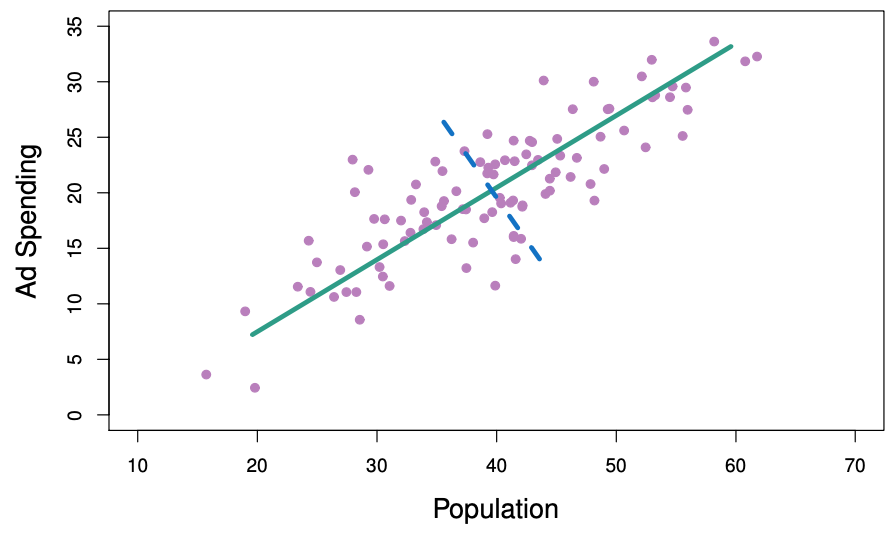
\includegraphics[width=3.33333in,height=\textheight]{images/first_component.png}

}

\end{figure}
\end{column}

\begin{column}{0.4\textwidth}
\begin{enumerate}
\item
  The first principal component is in the widest or most variable
  direction of the data.
\item
  It is also the line in the 2-dimensional space that is closest to the
  observations.
\end{enumerate}
\end{column}
\end{columns}
\end{frame}

\begin{frame}{The Second Principal Component}
\protect\hypertarget{the-second-principal-component}{}
Once we have found the first principal component \(Z_1\), the second
principal component \(Z_2\) can be found.

\alert{$Z_2$ is the linear combination of the features that again maximizes variance but is also uncorrelated with $Z_1$}.

\begin{itemize}
\item
  The scores \(z_{12}, z_{22}, \ldots, z_{n 2}\) are of the form
  \[z_{i 2}=\phi_{12} x_{i 1}+\phi_{22} x_{i 2}+\cdots+\phi_{p 2} x_{i p}\]
\item
  \(Z_2\) is uncorrelated with \(Z_1\) means that the direction
  \(\phi_1\) is orthogonal (perperdicular) to the direction \(\phi_1\).
\end{itemize}
\end{frame}

\begin{frame}{The Second Principal Component}
\protect\hypertarget{the-second-principal-component-1}{}
A data set with two features (Population and Ad Spending) is plotted
below. The green curve is the first principal component and the dashed
blue curve is the second.

\begin{columns}[T]
\begin{column}{0.6\textwidth}
\begin{figure}

{\centering 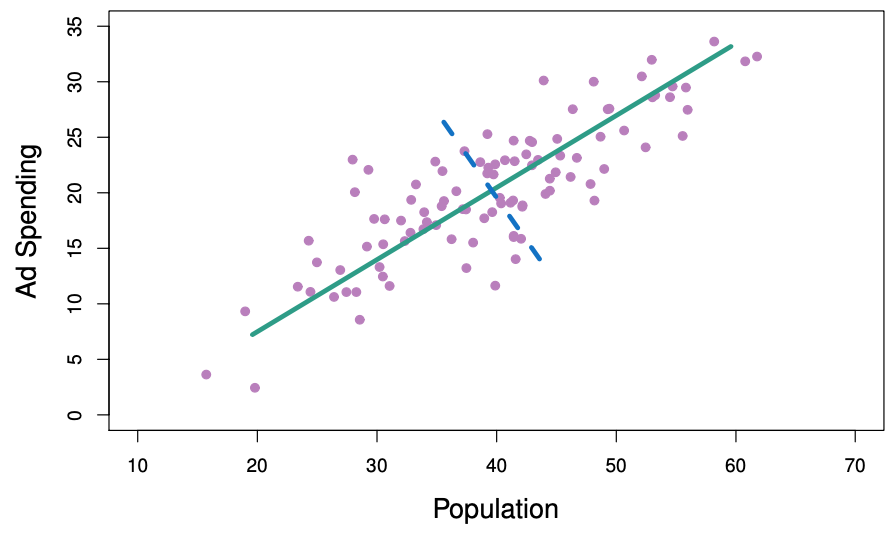
\includegraphics[width=3.33333in,height=\textheight]{images/first_component.png}

}

\end{figure}
\end{column}

\begin{column}{0.4\textwidth}
\begin{itemize}
\item
  The direction of the second principle component is perpendicular to
  the direction of the first principle component.
\item
  Since there are only two dimensions there is only one choice for
  \(\phi_2\).
\item
  If there were \(p > 2\) features, there would be multiple directions
  to choose between.
\end{itemize}
\end{column}
\end{columns}
\end{frame}

\begin{frame}{The Second Principal Component}
\protect\hypertarget{the-second-principal-component-2}{}
The three dimensional data set with the first and second principal
components defining the plane.

\begin{columns}[T]
\begin{column}{0.5\textwidth}
\begin{figure}

{\centering 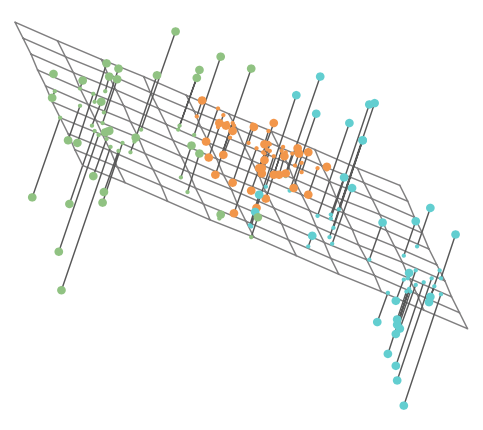
\includegraphics[width=2.92708in,height=\textheight]{images/second_component3D.png}

}

\end{figure}
\end{column}

\begin{column}{0.5\textwidth}
\begin{itemize}
\item
  The plane is as close to the data points as possible.
\item
  It also follows the directions along which the data varies the most.
\item
  The colour in this plot it not important.
\end{itemize}
\end{column}
\end{columns}
\end{frame}

\begin{frame}{Principal Component Analysis}
\protect\hypertarget{principal-component-analysis-1}{}
We can continue to create the principal components by taking the linear
combination of the features that maximizes variance while remaining
uncorrelated with the previous components.

\begin{itemize}
\item
  To make low-dimensional visualisations we can plot the scores for two
  principal components at a time.
\item
  Plot \(Z_1\) against \(Z_2\), \(Z_1\) against \(Z_3\), \(Z_2\) against
  \(Z_3\), and so on.
\item
  On the same plot we can plot the loading vectors on a different axis
  for each feature.
\item
  A plot with both the scores and loading vectors is called a biplot.
\end{itemize}
\end{frame}

\begin{frame}
\begin{columns}[T]
\begin{column}{0.6\textwidth}
\begin{figure}

{\centering 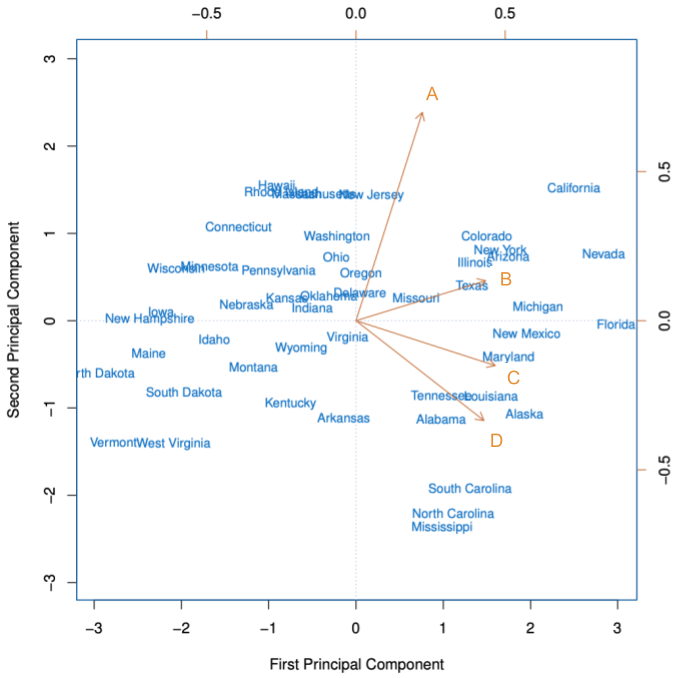
\includegraphics[width=2.91667in,height=\textheight]{images/PCA.png}

}

\end{figure}
\end{column}

\begin{column}{0.4\textwidth}
A biplot for the first two principal components of a data set of 50
states with features \{A, B, C, D\}. \newline

\begin{itemize}
\item
  The state names are the scores for the first two principal components.
\item
  The orange letters are the loadings for each of the features (top and
  right axis)
\item
  The loading for feature B is approximately

  \begin{itemize}
  \item
    0.54 on the first component (\(\phi_{B1} = 0.54\))
  \item
    0.17 on the first component (\(\phi_{B2} = 0.17\))
  \end{itemize}
\end{itemize}
\end{column}
\end{columns}
\end{frame}

\begin{frame}{The Proportion of Variance Explained}
\protect\hypertarget{the-proportion-of-variance-explained}{}
The plot we saw is a two-dimensional representation of a
four-dimensional data set.

\begin{itemize}
\item
  How much information have we lost?
\item
  How much of the variance in the data is not captured by the first few
  principal components?
\end{itemize}

\quad \(\Rightarrow\) We want to know the \textbf{proportion of variance
explained} (PVE) by each principal component.
\end{frame}

\begin{frame}{he Proportion of Variance Explained}
\protect\hypertarget{he-proportion-of-variance-explained}{}
Assuming that the features have been centered to have mean zero\ldots{}

\begin{itemize}
\item
  The \textbf{total variance} in a data set is:
  \[\sum_{j=1}^{p} \operatorname{Var}\left(X_{j}\right)=\sum_{j=1}^{p} \frac{1}{n} \sum_{i=1}^{n} x_{i j}^{2}\]
\item
  The variance explained by the \(m\)th principal component is:
  \[\frac{1}{n} \sum_{i=1}^{n} z_{i m}^{2}=\frac{1}{n} \sum_{i=1}^{n}\left(\sum_{j=1}^{p} \phi_{j m} x_{i j}\right)^{2}\]
\item
  The PVE of the \(m\)th principal component is:
  \[\frac{\sum_{i=1}^{n} z_{i m}^{2}}{\sum_{j=1}^{p} \sum_{i=1}^{n} x_{i j}^{2}}=\frac{\sum_{i=1}^{n}\left(\sum_{j=1}^{p} \phi_{j m} x_{i j}\right)^{2}}{\sum_{j=1}^{p} \sum_{i=1}^{n} x_{i j}^{2}}\]
\end{itemize}
\end{frame}

\begin{frame}{The Proportion of Variance Explained}
\protect\hypertarget{the-proportion-of-variance-explained-1}{}
\begin{itemize}
\item
  The cumulative PVE of the first \(M\) principal components is the sum
  of the first \(M\) PVEs.
\item
  There can be at most \(\min(n-1, p)\) principal components.
\item
  The sum of the PVEs for all the principal components sums to one.
\item
  In the US state plot shown previously:

  \begin{itemize}
  \item
    The first principal component accounts for 60\% of the variance in
    the data.
  \item
    The second principal component accounts for 25\% of the variance in
    the data.
  \item
    Together they account for 87\% of the variance in the data.
  \end{itemize}
\end{itemize}
\end{frame}

\begin{frame}{Scaling the Features}
\protect\hypertarget{scaling-the-features}{}
\alert{We scale each feature to have mean zero and standard deviation one before performing PCA.}

\begin{columns}[T]
\begin{column}{0.7\textwidth}
\begin{figure}

{\centering 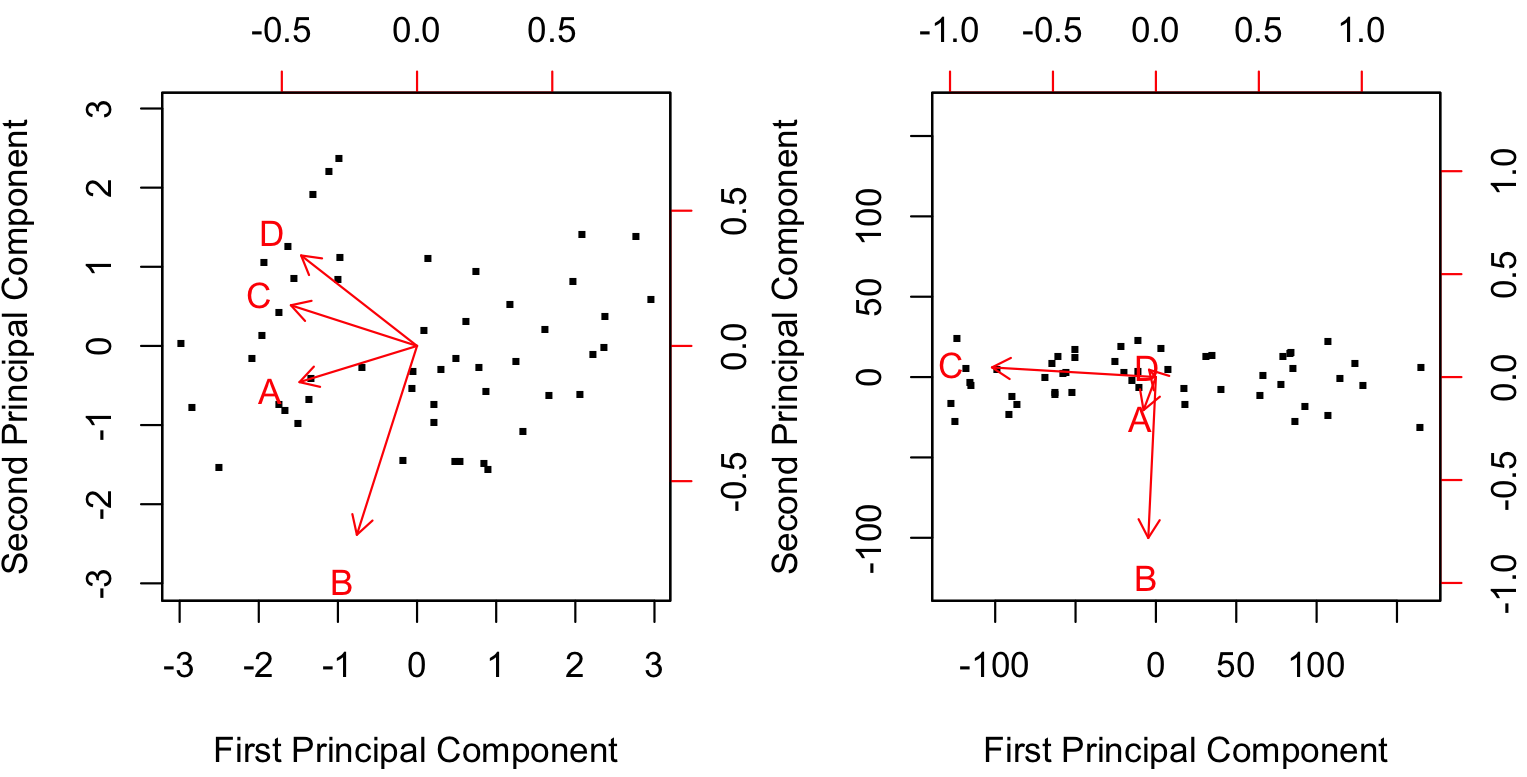
\includegraphics[width=4.16667in,height=\textheight]{images/scaled_sunscaled.png}

}

\end{figure}
\end{column}

\begin{column}{0.3\textwidth}
\begin{itemize}
\item
  Left: PCA biplot with variables scaled.
\item
  Right: Same data set but the variables have not been scaled.

  \begin{itemize}
  \item
    \(\phi_1\) is mostly C.
  \item
    \(\phi_2\) is mostly B.
  \end{itemize}
\item
  The right plot does not show patterns as well.
\end{itemize}
\end{column}
\end{columns}
\end{frame}

\begin{frame}{Uniqueness of the Principal Components}
\protect\hypertarget{uniqueness-of-the-principal-components}{}
\alert{Each principal component loading vector is unique up to a sign flip.}

\begin{itemize}
\item
  The loading vector specifies a direction in the \(p\)-dimensional
  space.
\item
  Changing the sign of every element in the loading vector does not
  change the direction.
\end{itemize}

\alert{The score vectors are unique up to a sign flip.}

\begin{itemize}
\tightlist
\item
  \(Z_1\) has the same variance as \(Z_2\).
\end{itemize}
\end{frame}

\begin{frame}{How Many Principal Components to Use}
\protect\hypertarget{how-many-principal-components-to-use}{}
\begin{itemize}
\item
  For a \(n \times p\) data matrix \(\mathbf{X}\) there are
  \(\min(n-1, p)\) distinct principal components.
\item
  \alert{Use the smallest number of principal components needed for a good understanding of the data.}
\item
  This will depend on the question and the data.

  \begin{itemize}
  \item
    Look at the first few principal components for patterns in the data.
  \item
    If there are none then the subsequent principal components will
    likely not help.
  \item
    If there are then look at the next principal components.
  \end{itemize}
\item
  Alternatively, use a \textbf{scree plot} to decide.

  \begin{itemize}
  \item
    Plot of the proportion of variance explained versus the number of
    principal components
  \item
    Find the point where the the PVE is minimal for subsequent principal
    components.
  \end{itemize}
\item
  Both methods are subjective which is why PCA is mostly used for
  exploratory data analysis.
\end{itemize}
\end{frame}

\begin{frame}{Scree Plot}
\protect\hypertarget{scree-plot}{}
\begin{columns}[T]
\begin{column}{0.5\textwidth}
\begin{figure}

{\centering 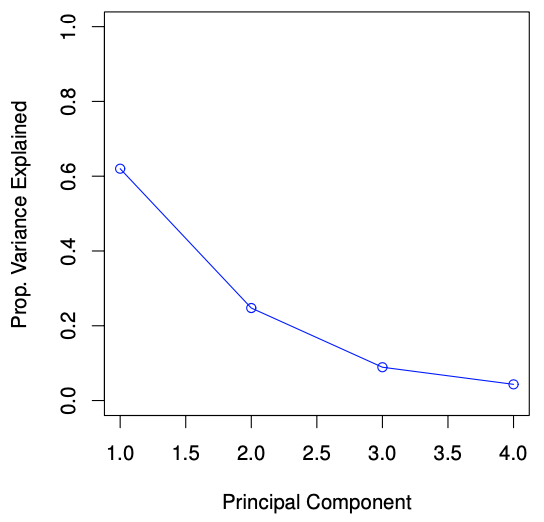
\includegraphics[width=2.71875in,height=\textheight]{images/scree_plot.png}

}

\end{figure}
\end{column}

\begin{column}{0.5\textwidth}
\begin{itemize}
\item
  Most of the variance is explained by the first two principal
  components.
\item
  The PVE levels off after this.
\item
  The third principal component accounts for less than 10\% of the
  variance in the data.
\item
  2 principal components are probably sufficient to get a good
  understanding of this data set.
\end{itemize}
\end{column}
\end{columns}
\end{frame}

\begin{frame}{Exercises: Principal Components Analysis}
\protect\hypertarget{exercises-principal-components-analysis}{}
Open the Unsupervised Learning Exercises R Markdown file.

\begin{itemize}
\tightlist
\item
  Go over the ``Principal Components Analysis'' section together as a
  class.
\end{itemize}
\end{frame}

\begin{frame}{Missing Values and Matrix Completion}
\protect\hypertarget{missing-values-and-matrix-completion}{}
The statistical learning methods we have learned in this course cannot
handle missing predictor values. What can we do?

\begin{itemize}
\item
  Remove rows that contain missing values.
\item
  If \(x_{ij}\) is missing, replace it with the mean of the \(j\)th
  predictor.
\item
  Perform \textbf{matrix completion} which uses principal components to
  impute the missing values.
\end{itemize}

The first two methods are convenient but they do not exploit the
correlation between the variables.
\end{frame}

\begin{frame}{Matrix Completion}
\protect\hypertarget{matrix-completion}{}
\alert{Matrix completion can only be used when the reason for missing data is random.}

\begin{itemize}
\item
  Random: a patient's weight is missing from the data set because the
  scale battery died.
\item
  Not random: a patient's weight is missing because they are too heavy
  for the scale.
\end{itemize}

Matrix completion works by
\alert{simultaneously estimating the missing values and solving the principal components}
iteratively. We will not cover the algorithm but if you are interested
see section 12.3 of ISLR2.
\end{frame}

\begin{frame}{Exercises: Matrix Completion}
\protect\hypertarget{exercises-matrix-completion}{}
Open the Unsupervised Learning Exercises R Markdown file.

\begin{itemize}
\tightlist
\item
  Go over the ``Matrix Completion'' section together as a class.
\end{itemize}
\end{frame}

\begin{frame}{Clustering Methods}
\protect\hypertarget{clustering-methods}{}
Both PCA and clustering are unsupervised learning methods that attempt
to simplify the data via summaries.

\begin{itemize}
\item
  \alert{Clustering methods aim to find subgroups (clusters) in a data set.}
\item
  Observations within a cluster are similar to each other and
  observations from different clusters are quite different.
\item
  The definitions of similar and different depend on the problem at
  hand.
\end{itemize}

There are many clustering methods but we will cover the two best-known:

\begin{itemize}
\item
  \(K\)-means clustering
\item
  Hierarchical clustering
\end{itemize}
\end{frame}

\begin{frame}{\(K\)-Means Clustering}
\protect\hypertarget{k-means-clustering}{}
\alert{$K$-means clustering seeks to partition a data set into $K$ distinct, non-overlapping clusters.}

\begin{enumerate}
\item
  Specify the desired number of clusters \(K\).
\item
  Use the \(K\)-means algorithm to assign each observation to a cluster.
\end{enumerate}

We need some notation:

\begin{itemize}
\item
  \(C_1, \dots, C_K\) are the sets containing the indices of the
  observations in each cluster. \emph{(Ex: if the} \(i\)th observation
  is in the \(k\)th cluster then \(i \in C_k\))

  \begin{itemize}
  \item
    Every observation belongs to a cluster.
  \item
    No observation belongs to more than one cluster.
  \end{itemize}
\end{itemize}

Want to
\alert{choose clusters that minimize the \textbf{within-cluster variation}}
\(W(C_k)\) for all clusters \(C_k\).

\(\rightarrow\) Minimize the amount by which observations within a
cluster differ.
\end{frame}

\begin{frame}{Within-Cluster Variation}
\protect\hypertarget{within-cluster-variation}{}
Within-Cluster variation for the \(k\)th cluster is the
\alert{sum of the pairwise squared Euclidean distances between each observation in the $k$th cluster, divided by the number of observations in the cluster}
(\(|C_k|\)). That is,
\[W\left(C_{k}\right)=\frac{1}{\left|C_{k}\right|} \sum_{i, i^{\prime} \in C_{k}} \sum_{j=1}^{p}\left(x_{i j}-x_{i^{\prime} j}\right)^{2}\]

The \textbf{Euclidean distance} is a way to measure distance in
\(p\)-dimensional space. Suppose we have
\(\mathbf{x} = (x_1, \dots, x_p)\) and
\(\mathbf{y} = (y_1, \dots, y_p)\), then the Euclidean distance is
\[d(\mathbf{x}, \mathbf{y}) = \sqrt{(x_1 - y_1)^2 + \cdots + (x_p - y_p)^2}\]
Note that we use the squared Euclidean distance in \(W(C_k)\) so we
remove the square-root.
\end{frame}

\begin{frame}{Within-Cluster Variation}
\protect\hypertarget{within-cluster-variation-1}{}
To minimize within-cluster variation in all the \(K\) clusters we need
to solve \[
\underset{C_{1}, \ldots, C_{K}}{\operatorname{minimize}}\left\{\sum_{k=1}^{K} \frac{1}{\left|C_{k}\right|} \sum_{i, i^{\prime} \in C_{k}} \sum_{j=1}^{p}\left(x_{i j}-x_{i^{\prime} j}\right)^{2}\right\}
\] We use the \(K\)-means clustering algorithm!
\end{frame}

\begin{frame}{K-Means Clustering Algorithm}
\protect\hypertarget{k-means-clustering-algorithm}{}
\begin{block}{K-Means Clustering Algorithm}
\protect\hypertarget{k-means-clustering-algorithm-1}{}
\begin{enumerate}
\item
  Randomly assign each observation a number between 1 and \(K\). These
  are the initial cluster assignments.
\item
  Repeat steps below until cluster assignments are static.
\end{enumerate}

\begin{itemize}
\item
  For each cluster compute the cluster \textbf{centroid}. The \(k\)th
  cluster centroid is the \(p\) dimensional vector of the feature means
  for the observations in the \(k\)th cluster.
\item
  Assign each observation to the cluster with the closest centroid.
\end{itemize}

The results obtained depend on the initial random cluster assignment in
step 1 of the algorithm.
\end{block}
\end{frame}

\begin{frame}{Means Clustering Algorithm}
\protect\hypertarget{means-clustering-algorithm}{}
The \(K\)-means algorithm finds a \textbf{local optimum} which does not
guarantee it is the \textbf{global optimum}.

\begin{columns}[T]
\begin{column}{0.6\textwidth}
\begin{figure}

{\centering 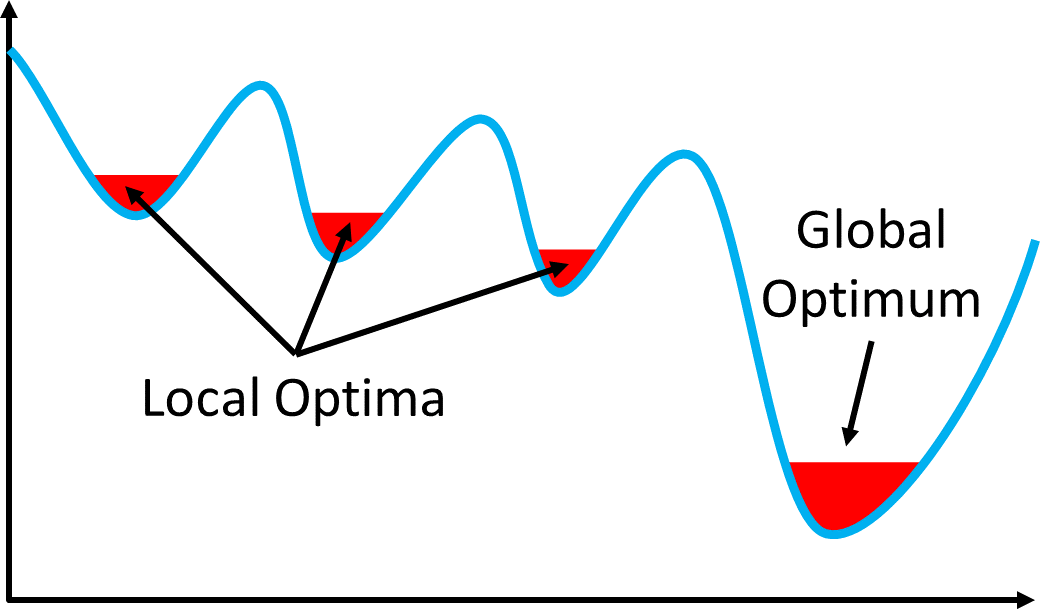
\includegraphics[width=3.125in,height=\textheight]{images/Local-Global-Optimum.png}

}

\end{figure}
\end{column}

\begin{column}{0.4\textwidth}
To find the global optima:

\begin{exampleblock}{}
\begin{enumerate}
    \item Run the algorithm multiple times with random initial cluster assignments.
    \item Choose the clustering that minimizes the within-cluster variation (1).
\end{enumerate}
\end{exampleblock}
\end{column}
\end{columns}
\end{frame}

\begin{frame}{Exercises: K-Means Clustering}
\protect\hypertarget{exercises-k-means-clustering}{}
Open the Unsupervised Learning Exercises R Markdown file.

\begin{itemize}
\tightlist
\item
  Go over the ``K-Means Clustering'' section together as a class.
\end{itemize}
\end{frame}

\begin{frame}{Dendrogram}
\protect\hypertarget{dendrogram}{}
\begin{columns}[T]
\begin{column}{0.5\textwidth}
\begin{figure}

{\centering 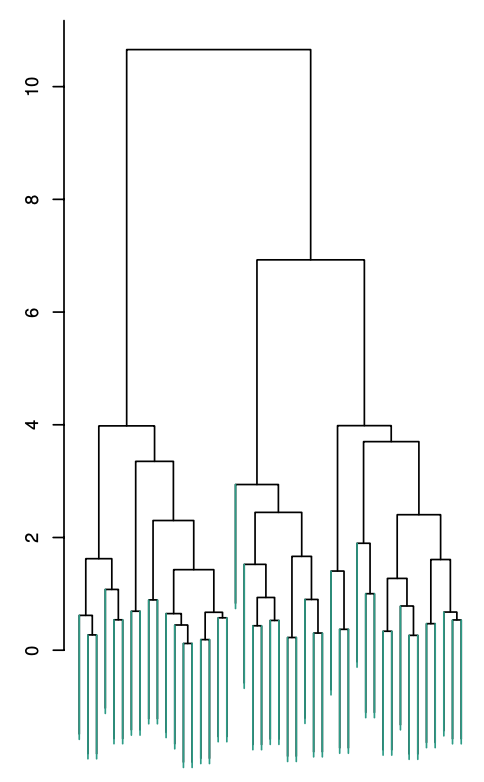
\includegraphics[width=1.80208in,height=\textheight]{images/dendrogram.png}

}

\end{figure}
\end{column}

\begin{column}{0.5\textwidth}
Hierarchical clustering results in a \textbf{dendrogram} which is a
tree-based representation of the observations.

\begin{itemize}
\item
  Each leaf (green stick) is an observation.
\item
  As we move up the dendrogram, observations that are similar fuse into
  branches.
\item
  Then branches fuse into other branches which indicates that the groups
  of observations are similar.
\item
  \alert{The height at which two observations fuse indicates how different the two observations are.}
\end{itemize}
\end{column}
\end{columns}
\end{frame}

\begin{frame}{Dendrogram}
\protect\hypertarget{dendrogram-1}{}
\begin{columns}[T]
\begin{column}{0.5\textwidth}
\begin{figure}

{\centering 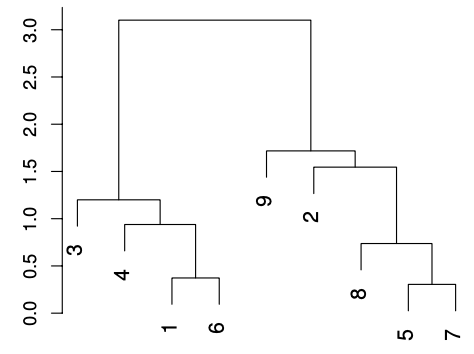
\includegraphics[width=3.14583in,height=\textheight]{images/small_dendogram.png}

}

\end{figure}
\end{column}

\begin{column}{0.5\textwidth}
\begin{itemize}
\item
  Observations 1 and 6 are quite similar since they fuse at the bottom
  of the dendrogram.
\item
  Observations 9 and 2 are quite dissimilar since they fuse near the
  top.
\item
  Observation 9 is equally similar to observations 2, 8, 5, and 7.
\item
  Thus, the horizontal axis tells us nothing about similarity.
\end{itemize}
\end{column}
\end{columns}
\end{frame}

\begin{frame}{Clustering with a Dendrogram}
\protect\hypertarget{clustering-with-a-dendrogram}{}
\alert{To create clusters we make a horizontal cut across the dendrogram. The distinct sets of observations beneath the cut are the clusters.}

\begin{columns}[T]
\begin{column}{0.5\textwidth}
\begin{figure}

{\centering 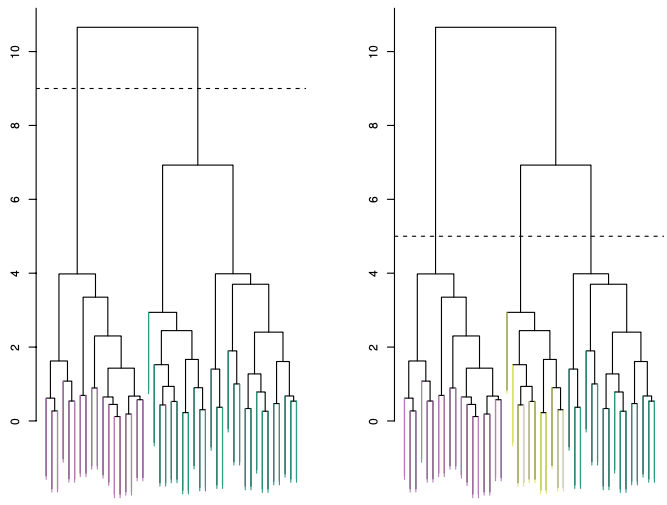
\includegraphics[width=3.125in,height=\textheight]{images/hierarchical_cluster.png}

}

\end{figure}
\end{column}

\begin{column}{0.5\textwidth}
\begin{itemize}
\item
  Left: Cutting at a height of 9 results in two clusters.
\item
  Right: Cutting at a height of 5 results in three clusters.
\item
  We can obtain any number of clusters from a single dendrogram.
\item
  Usually the height of the cut is selected by eye based on the desired
  number of clusters.
\end{itemize}
\end{column}
\end{columns}
\end{frame}

\begin{frame}{Dissimilarity Measures}
\protect\hypertarget{dissimilarity-measures}{}
In order to create a dendrogram, we need to define measures of
dissimilarity between:

\begin{itemize}
\item
  A pair of observations.
\item
  A pair of groups of observations.
\end{itemize}

The choice of dissimilarity measures have a strong influence on the
shape of the dendrogram. The type of data and the question at hand
should be considered.
\end{frame}

\begin{frame}{Dissimilarity Between Observations}
\protect\hypertarget{dissimilarity-between-observations}{}
The most common choice for dissimilarity between observations is
\textbf{Euclidean distance}.

\begin{itemize}
\tightlist
\item
  Observations that are close to each other are similar.
\end{itemize}

But in some cases, \textbf{correlation-based distance} might be
preferred.

\begin{itemize}
\item
  Observations with features that are highly correlated are similar.
\item
  This focuses on the shapes of the observation profiles rather than
  their magnitudes.
\end{itemize}
\end{frame}

\begin{frame}{Linkage}
\protect\hypertarget{linkage}{}
Linkage refers to the dissimilarity between two groups of observations.
The four most common types of linkage are:

\begin{itemize}
\item
  \textbf{Complete}
\item
  \textbf{Single}
\item
  \textbf{Average}
\item
  \textbf{Centroid}
\end{itemize}
\end{frame}

\begin{frame}{Complete Linkage}
\protect\hypertarget{complete-linkage}{}
\textbf{Complete linkage} measures maximal intercluster dissimilarity.

\begin{block}{\quad}
\protect\hypertarget{section}{}
\begin{enumerate}
\item
  Compute all pairwise dissimilarities between the observations in
  cluster A and cluster B.
\item
  Record the largest of these dissimilarities.
\end{enumerate}
\end{block}
\end{frame}

\begin{frame}{Single Linkage}
\protect\hypertarget{single-linkage}{}
\textbf{Single linkage} measures minimal intercluster dissimilarity.

\begin{enumerate}
\item
  Compute all pairwise dissimilarities between the observations in
  cluster A and cluster B.
\item
  Record the smallest of these dissimilarities.
\end{enumerate}

This type of linkage can result in trailing clusters in which a single
observation is fused at a time. (i.e.~leaves fuse to branches more often
than branches fuse to branches)
\end{frame}

\begin{frame}{Average Linkage}
\protect\hypertarget{average-linkage}{}
\textbf{Average linkage} measures mean intercluster dissimilarity.

\begin{block}{\quad}
\protect\hypertarget{section-1}{}
\begin{enumerate}
\item
  Compute all pairwise dissimilarities between the observations in
  cluster A and cluster B.
\item
  Record the average of these dissimilarities.
\end{enumerate}
\end{block}
\end{frame}

\begin{frame}{Complete Linkage}
\protect\hypertarget{complete-linkage-1}{}
\textbf{Centroid linkage} measures intercluster centroid dissimilarity.

\begin{block}{\quad}
\protect\hypertarget{section-2}{}
\begin{enumerate}
\tightlist
\item
  Compute the dissimilarity of the centroid for cluster A (a vector of
  the feature means) and the centroid for cluster B.
\end{enumerate}

Centroid linkage can result in \textbf{inversion} whereby two clusters
are fused at a height below either of the individual clusters.
\end{block}
\end{frame}

\begin{frame}{Hierarchical Clustering Algorithm}
\protect\hypertarget{hierarchical-clustering-algorithm}{}
\begin{block}{Hierarchical Clustering Algorithm}
\protect\hypertarget{hierarchical-clustering-algorithm-1}{}
\begin{enumerate}
\item
  Treat each of the \(n\) observations are its own cluster.
\item
  Compute the pairwise dissimilarity between each observation.
\item
  For \(i = n, n-1, \dots, 2\):
\end{enumerate}

\begin{itemize}
\item
  Identify the pair of clusters that are the least dissimilar among the
  \(i\) clusters.
\item
  Fuse these two clusters in the dendrogram at the height that indicates
  their dissimilarity.
\item
  Compute the new pairwise inter-cluster dissimilarities among the
  \(i - 1\) remaining clusters.
\end{itemize}
\end{block}
\end{frame}

\begin{frame}{Hierarchial Clustering Algorithim}
\protect\hypertarget{hierarchial-clustering-algorithim}{}
The first iteration of the algorithm on a data set of 9 observations
with two features. Euclidean distance and complete linkage are used.

\begin{columns}[T]
\begin{column}{0.7\textwidth}
\begin{figure}

{\centering 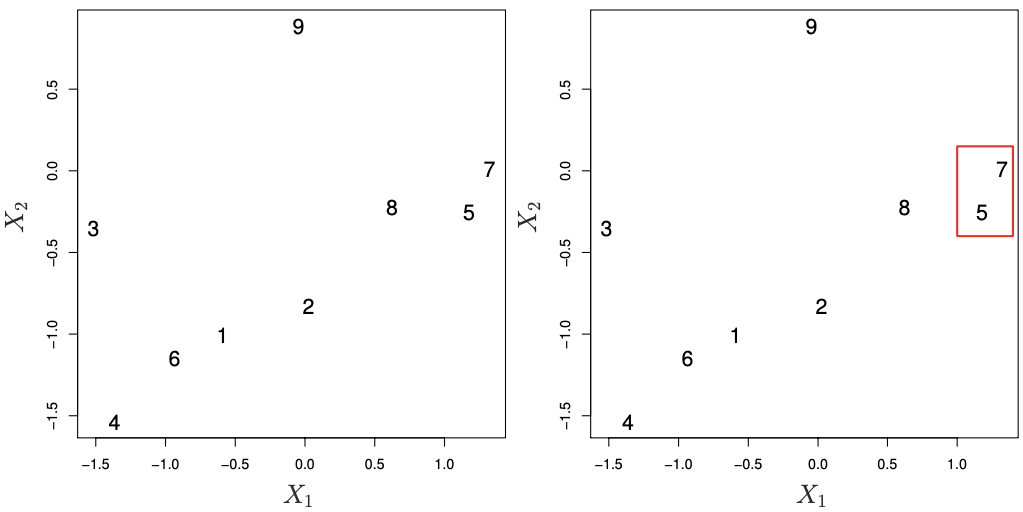
\includegraphics[width=4.27083in,height=\textheight]{images/hierarchical_alg1.png}

}

\end{figure}
\end{column}

\begin{column}{0.3\textwidth}
\begin{itemize}
\item
  Left: there are 9 clusters each containing one observation.
\item
  Right: identify \{7\} and \{5\} as the most similar clusters and fuse
  them.
\end{itemize}
\end{column}
\end{columns}
\end{frame}

\begin{frame}{Hierarchial Clustering Algorithim}
\protect\hypertarget{hierarchial-clustering-algorithim-1}{}
The next 2 iterations of step 3 of the algorithm.

\begin{columns}[T]
\begin{column}{0.7\textwidth}
\begin{figure}

{\centering 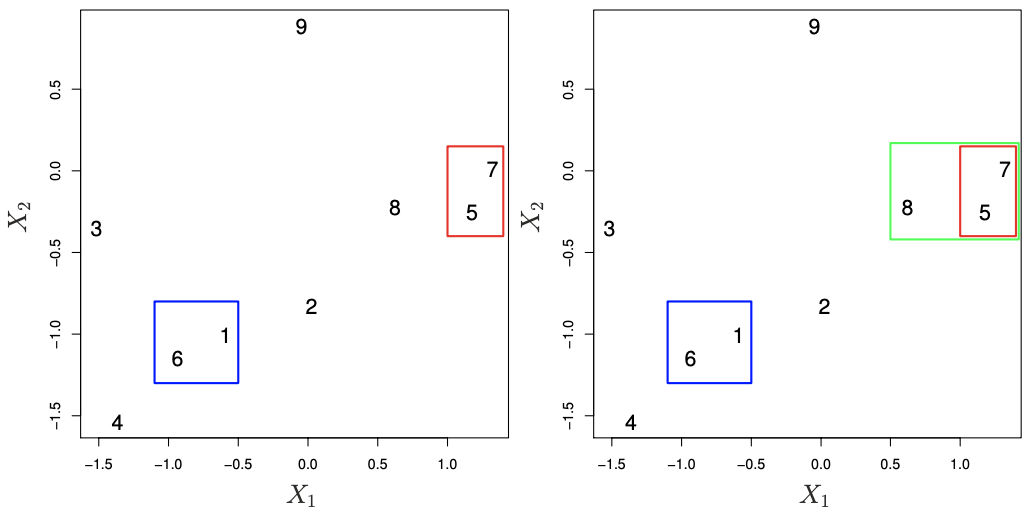
\includegraphics[width=4.27083in,height=\textheight]{images/hierarchical_alg2.png}

}

\end{figure}
\end{column}

\begin{column}{0.3\textwidth}
\begin{itemize}
\item
  Left: there are 9 clusters each containing one observation.
\item
  Right: identify \{7\} and \{5\} as the most similar clusters and fuse
  them.
\end{itemize}
\end{column}
\end{columns}
\end{frame}

\begin{frame}{Linkage}
\protect\hypertarget{linkage-1}{}
The choice of the linkage type will have an effect on the dendrogram
produced by the hierarchical clustering algorithm.

\begin{figure}

{\centering 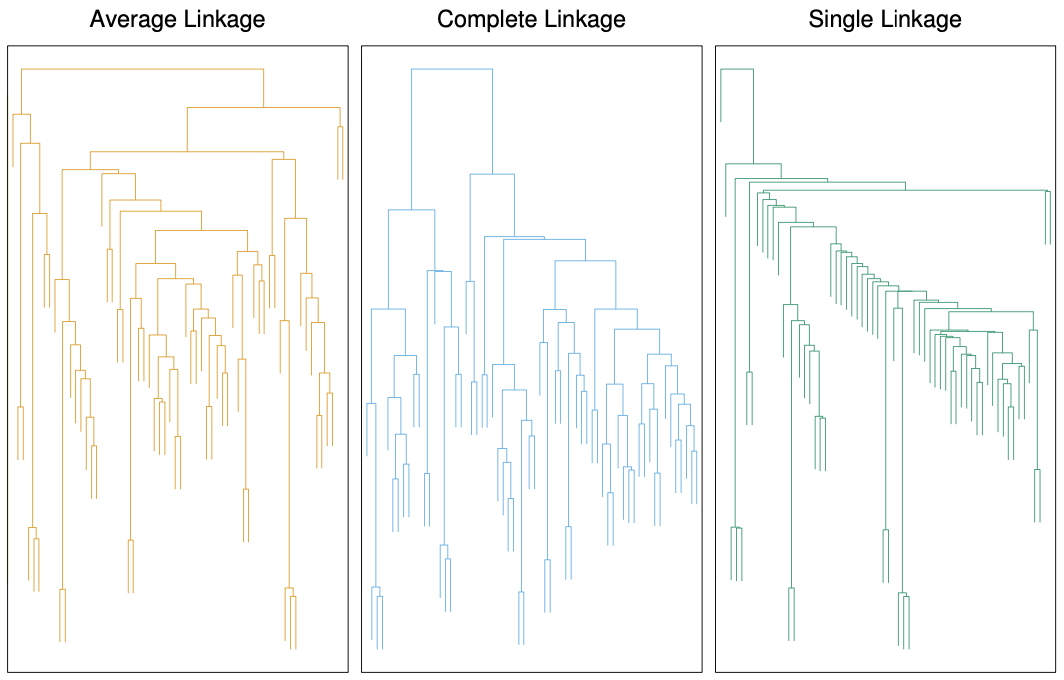
\includegraphics[width=3.59375in,height=\textheight]{images/linkage_choice.png}

}

\end{figure}
\end{frame}

\begin{frame}{Exercises: Hierarchical Clustering}
\protect\hypertarget{exercises-hierarchical-clustering}{}
Open the Unsupervised Learning Exercises R Markdown file.

\begin{itemize}
\tightlist
\item
  Go over the ``Hierarchical Clustering'' section together as a class.
\end{itemize}
\end{frame}

\begin{frame}{References}
\protect\hypertarget{references}{}
Chapter 12 of the ISLR2 book:

\quad James, Gareth, et al.~``Unsupervised Learning.'' An Introduction
to Statistical Learning:

\quad with Applications in R, 2nd ed., Springer, 2021.

Local optima photo:

\quad By Christoph Roser at AllAboutLean.com under the free CC-BY-SA 4.0
license.
\end{frame}



\end{document}
